\documentclass{lni}

\IfFileExists{latin1.sty}{\usepackage{latin1}}{\usepackage{isolatin1}}

\usepackage{graphicx}
\usepackage{color}

\author{Andreas Kn�pfle \& Tobias Schmid \\\\andreas.knoepfle@fu-berlin.de, tobias.schmid@fu-berlin.de}
\title{Eigennamenerkennung in mathematischen Texten}
\begin{document}
\maketitle

\begin{abstract}
abstract
\end{abstract}

\tableofcontents

\section{Einleitung}

Mit Hilfe einer Eigennamenerkennung ist es m�glich Eigennamen in Texten zu finden. Es k�nnte beispielsweise interessant sein alle Personennamen in einem Text zu finden, um schnell herauszufinden, um wen es in diesem Text geht. Unterschiedliche Dom�nen haben meist auch unterschiedliche Eigennamen. In den einzelnen Dom�nen, wie z.B. die Mathematik, entstehen Eigennamen auf unterschiedliche Weisen. Wenn beispielsweise ein bekannter Mathematiker einen neuen Algorithmus entwickelt, so wird dieser oft nach dem Namen des Mathematikers benannt. Jedoch gibt es in den meisten F�llen keine eindeutigen Regeln, nach welchen Eigennamen entstehen und es ist somit nicht trivial diese Eigennamen in Texten zu finden. Eine Eigennamenerkennung aus einer bestimmten Dom�ne (z.B. die Biologie), funktioniert vermutlich auch nicht problemlos in einer anderen Dom�ne.\\

Es gibt schon verschiedene Eigennamenerkennungen in unterschiedlichen Dom�nen. Jedoch gibt es auch einige Dom�nen, f�r welche es noch keine bzw. nur ungen�gend zufriedenstellende Eigennamenerkennungen gibt. Eine Dom�ne f�r welche es noch keine zufriedenstellende Eigennamenerkennung gibt, ist die Mathematik, mit welcher sich dieser Artikel besch�ftigt.


\section{Grundlagen}
In mathematischen Texten k�nnen Standart-Tools zur Erkennung von Eigennamen, wie die von Personen, Organisationen oder Orten nicht verwendet werden, da die in die Mathematik eigene Eigennamen definiert. Beispielsweise gibt es Formeln, Gleichungen oder Theoreme wie z.B. Satz des Pythagoras oder das Bayestheorem, die eigene Namen tragen und oft in mathematischen Texten vorkommen. Die Erkennung dieser Eigennamen wurde in dieser Arbeit mit zwei unterschiedlichen Ans�tzen implementiert:
\begin{itemize}
	\item Regelbasierte Erkennung 
	\item Maschinelles Lernen
\end{itemize}
Bestehende Werkzeuge zur Eigennamenerkennung k�nnen zus�tzlich zur eigentlichen Erkennung der Eigennamen Label vergeben, die die Erkannten Eigennamen typisieren (z.B. erhalten erkannte Personennamen ein Person-Label). Da es aber in der Mathematik sehr viele verschiedene Konzepte gibt und sich die mathematischen Eigennamen oft vielen Konzepten zuordnen lassen, wurde in dieser Arbeit auf eine zus�tzliche Labelung der Eigenamen verzichtet. Die implementierten Ans�tze verwenden daher jeweils ein gemeinsames Label "MATH" f�r mathematische Entit�ten.
\subsection{Architektur}

\begin{figure}
  \begin{center}
  	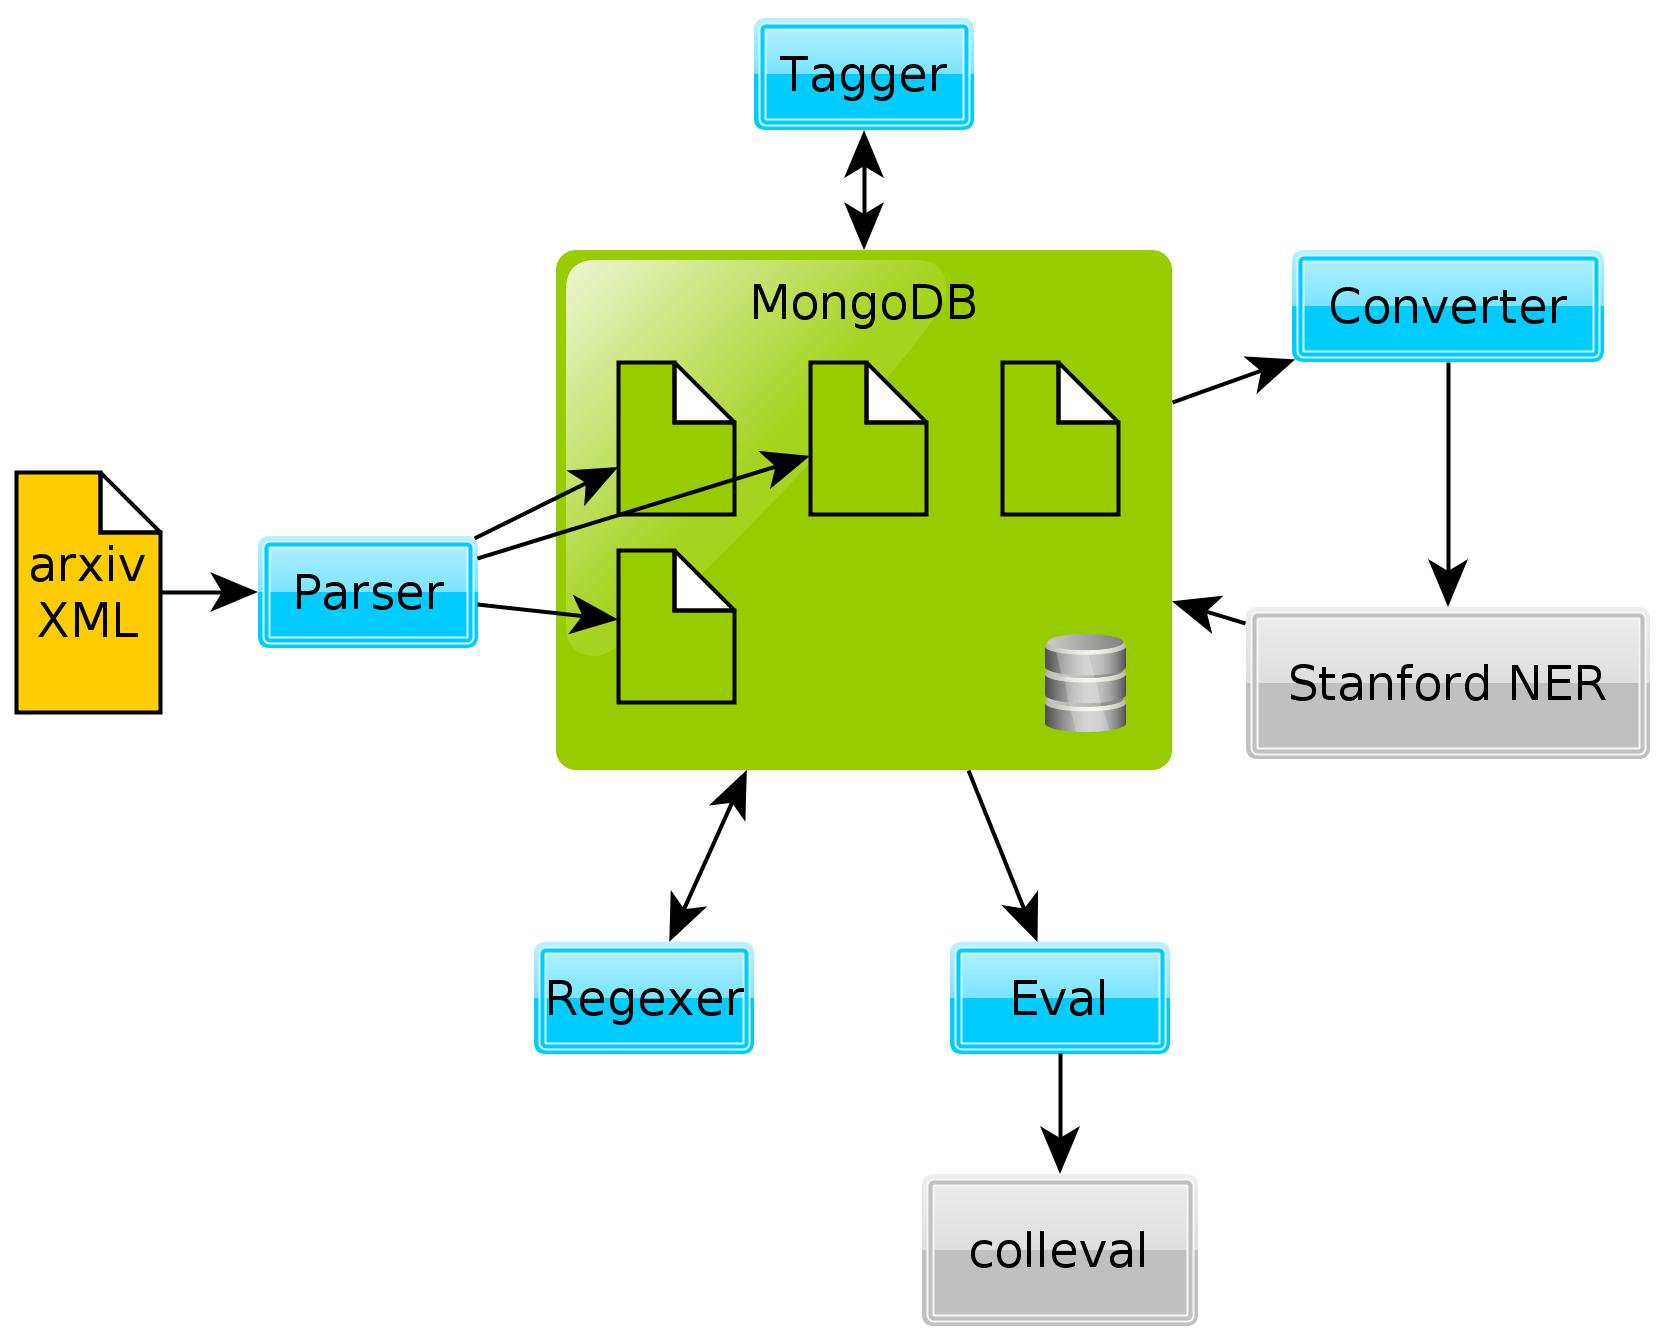
\includegraphics[width=0.7\textwidth]{image/arch.jpg}
  	\caption{Architektur der Evaluationsumgebung\label{arch}}
  \end{center}
\end{figure}


\subsection{Regelbasierte Erkennung}

\subsection{Erkennung mit maschinellem Lernen}

\subsection{Datensatz}


\subsection{Evaluationsmethoden}

F�r die Evaluation der Ergebnisse werden drei Ma�e verwendet:

\(Precision = \frac{Anzahl richtig getaggte Woerter}{Anzahl getaggte Woerter}\) 

\(Recall = \frac{Anzahl richtig getaggte Woerter}{Anzahl richtig getaggte Woerter + Anzahl nicht gefundene Woerter}\) 

\(F1 = 2 \cdot \frac{Precision \cdot Recall}{Precision + Recall}\)



\section{Analyse}

\subsection{Ergebnisse der Regelbasierte Erkennung}

Mit der Implementierung der regelbasierten Erkennung wurden folgende Ergebnisse erzielt:
\begin{list}{}{}
\item Precision:		95.27\% 
\item Recall:		49.55\% 
\item FB1-Ma�:			57.97 
\end{list}

Folgende Details liegen diesem Ergebnis zu grunde:
\begin{list}{}{}
\item Anzahl W�rter in Testdatei:     	10077
\item Anzahl W�rter mit Tags:               664
\item Anzahl NER-getaggte W�rter:           471
\item Anzahl richtig NER-getaggte W�rter:   329
\end{list}

\subsubsection*{Nicht erkannte Eigennamen}


\subsubsection*{Falsch erkannte Eigennamen}



\subsection{Ergebnisse der Erkennung mit maschinellem Lernen}

Mit der Implementierung der Erkennung mit maschinellem Lernen wurden folgende Ergebnisse erzielt:
\begin{list}{}{}
\item Precision:		90.36\% 
\item Recall:		64.13\% 
\item FB1-Ma�:		75.02
\end{list}

Folgende Details liegen diesem Ergebnis zu grunde:
\begin{list}{}{}
\item Anzahl W�rter in Testdatei:            11240
\item Anzahl W�rter mit Tags:                658
\item Anzahl NER-getaggte W�rter:            467
\item Anzahl richtig NER-getaggte W�rter:    422
\end{list}

\subsubsection*{Nicht erkannte Eigennamen}

There are 7622 isomorphism classes of smooth {\color{red}Fano polytopes} and 72256 isomorphism(...)

(...) quasi-isometric to {\color{red}Euclidean spaces} of arbitrary dimension ....

(...) is constructed based on {\color{red}L. Bers' theory of formal powers}.

(...) for the affine {\color{red}Weyl group symmetry}.   

(...) of equivariant {\color{green}Schubert classes} on {\color{red}Grassmannians} which implies(...)

(...) of the Fourier coefficients of {\color{green}Siegel modular} {\color{red}forms} on {\color{red}Maass Space} are obtained (...)

(...) modeling a {\color{green}Non-Newtonian fluid} {\color{red}of polymer aqueous solutions}.

(...) recall a {\color{red}theorem of Cantor} that (...) 

\subsubsection*{Falsch erkannte Eigennamen}

(...) the dual {\color{green}Feynman transform} {\color{red}whose algebras} are not necessarily (...)

(...) where {\color{green}Mathai's entropy} {\color{red}leads} to pathway (...)

(...) pricing continuous arithmetic average {\color{red}Asian options} in the (...)

(...) of the bacteria {\color{red}Staphylococcus aureus} in intermediate moisture (...)

(...) Food scientists at the {\color{red}U.S. Army's Natick Solider Center have} developed a model (...)

\section{Fazit}

\end{document}

